\documentclass{article}
\usepackage{titlesec}

\usepackage[citestyle=authortitle-terse]{biblatex}
\addbibresource{bibliography.bib}

\setcounter{secnumdepth}{0}
%\usepackage{sectsty}
%\sectionfont{\fontsize{17}{20}\selectfont}

\usepackage[left=4cm, right=4cm]{geometry}
\usepackage{palatino,eulervm,dutchcal,xcolor}%fonts
\usepackage{graphicx,subcaption,float}
\usepackage{enumitem,parskip,multicol}
\usepackage{amsthm,amssymb,amsmath,mathtools,thmtools}
\usepackage{tikz,tikz-cd}
\usetikzlibrary{%
	matrix,%
	calc,%
	arrows,%
	shapes,
	decorations.markings,backgrounds,calc,intersections}
\tikzcdset{scale cd/.style={every label/.append style={scale=#1},
		cells={nodes={scale=#1}}}}
\usepackage[bookmarks,bookmarksopen,bookmarksdepth=3]{hyperref}
\hypersetup{%colores
	colorlinks=true,
	urlcolor=blue,
	linkcolor=magenta,
	citecolor=blue,
	filecolor=blue,
	urlbordercolor=white,
	linkbordercolor=white,
	citebordercolor=white,
	filebordercolor=white}
\usepackage{cleveref}
\Crefname{exercise}{Exercise}{Exercises}

\newcommand{\fakesection}[1]{%
	\par\refstepcounter{section}% Increase section counter
	\sectionmark{#1}% Add section mark (header)
	\addcontentsline{toc}{section}{\protect\numberline{\thesection}#1}% Add section to ToC
	% Add more content here, if needed.
}

\makeatletter %Hide section number
\def\@seccntformat#1{%
	\expandafter\ifx\csname c@#1\endcsname\c@section\else
	\csname the#1\endcsname\quad
	\fi}
\makeatother

\definecolor{blue-violet}{rgb}{0.54, 0.17, 0.89}
\definecolor{azure}{rgb}{0.0, 0.5, 1.0}
\definecolor{green(ncs)}{rgb}{0.0, 0.62, 0.42}
\definecolor{forestgreen}{rgb}{0.13, 0.55, 0.13}
\definecolor{limegreen}{rgb}{0.2, 0.8, 0.2}
\definecolor{palatinateblue}{rgb}{0.15, 0.23, 0.89}
\definecolor{trueblue}{rgb}{0.0, 0.45, 0.81}
\definecolor{goldenyellow}{rgb}{1.0, 0.87, 0.0}
\definecolor{fashionfuchsia}{rgb}{0.96, 0.0, 0.63}
\definecolor{brightcerulean}{rgb}{0.11, 0.67, 0.84}
\definecolor{jonquil}{rgb}{0.98, 0.85, 0.37}
\definecolor{lavendermagenta}{rgb}{0.93, 0.51, 0.93}
\definecolor{peru}{rgb}{0.8, 0.52, 0.25}
\definecolor{persimmon}{rgb}{0.93, 0.35, 0.0}
\definecolor{persianred}{rgb}{0.8, 0.2, 0.2}
\definecolor{persianblue}{rgb}{0.11, 0.22, 0.73}
\definecolor{persiangreen}{rgb}{0.0, 0.65, 0.58}
\definecolor{persianyellow}{rgb}{0.9, 0.89, 0.0}

\declaretheoremstyle[headfont=\color{trueblue}\normalfont\bfseries,]{colored1}
\declaretheoremstyle[headfont=\color{forestgreen}\normalfont\bfseries,]{colored2}
\declaretheoremstyle[headfont=\color{peru}\normalfont\bfseries,]{colored3}
\declaretheoremstyle[headfont=\color{persiangreen}\normalfont\bfseries,]{colored4}
\declaretheoremstyle[headfont=\color{brightcerulean}\normalfont\bfseries,]{colored5}
\declaretheoremstyle[headfont=\color{lavendermagenta}\normalfont\bfseries,]{colored6}
\declaretheoremstyle[headfont=\color{blue-violet}\normalfont\bfseries,]{colored7}
\declaretheoremstyle[headfont=\color{green(ncs)}\normalfont\bfseries,]{colored8}
\declaretheoremstyle[headfont=\color{peru}\normalfont\bfseries,]{colored9}
\declaretheoremstyle[headfont=\color{persiangreen}\normalfont\bfseries,]{colored10}
\declaretheoremstyle[headfont=\color{red}\normalfont\bfseries,]{colored11}

\declaretheorem[style=colored1,numberwithin=section,name=Theorem]{thm}
\declaretheorem[style=colored1,numbered=no,name=Proposition]{prop}
\declaretheorem[style=colored3,numberwithin=section,numberlike=thm,name=Lemma]{lemma}
\declaretheorem[style=colored4,numberwithin=section,numberlike=thm,name=Corollary]{coro}
\declaretheorem[style=colored5,numbered=no,name=Example]{example}
\declaretheorem[style=colored5,numbered=no,name=Examples]{exemplos}
\declaretheorem[style=colored7,numberwithin=section,name=Exercise]{exercise}
\declaretheorem[style=colored9,numbered=no,name=Remark]{remark}
\declaretheorem[style=colored9,numbered=no,name=Claim]{claim}
\declaretheorem[style=colored8,numbered=no,name=Definition]{defn}
\declaretheorem[style=colored11,numbered=no,name=Question]{question}

\newcommand{\R}{\mathbb{R}}
\newcommand{\Z}{\mathbb{Z}}
\newcommand{\N}{\mathbb{N}}
\newcommand{\C}{\mathbb{C}}
\newcommand{\Q}{\mathbb{Q}}
\newcommand{\D}{\mathbb{D}}
\newcommand{\T}{\mathbb{T}}
\renewcommand{\P}{\mathbb{P}}
\renewcommand{\H}{\mathbb{H}}
\newcommand{\Ac}{\mathcal{A}}
\newcommand{\Bc}{\mathcal{B}}
\newcommand{\Cc}{\mathcal{C}}
\newcommand{\Dc}{\mathcal{D}}
\newcommand{\Ec}{\mathcal{E}}
\newcommand{\Fc}{\mathcal{F}}
\newcommand{\Gc}{\mathcal{G}}
\newcommand{\Lc}{\mathcal{L}}
\newcommand{\Oc}{\mathcal{O}}
\newcommand{\Qc}{\mathcal{Q}}
\newcommand{\Sc}{\mathcal{S}}
\newcommand{\Wc}{\mathcal{W}}
\newcommand{\mf}{\mathfrak{m}}
\newcommand{\gf}{\mathfrak{g}}
\newcommand{\X}{\mathfrak{X}}
\newcommand{\hf}{\mathfrak{h}}
\newcommand{\glf}{\mathfrak{gl}}
\newcommand{\of}{\mathfrak{o}}

\renewcommand{\Im}{\operatorname{Im}}
\renewcommand{\O}{\operatorname{O}}
\renewcommand{\S}{\mathbb{S}}
\renewcommand{\T}{\mathbb{T}}
\DeclareMathOperator{\Lie}{\operatorname{Lie}}

\DeclareMathOperator{\img}{img}
\DeclareMathOperator{\Arg}{Arg}
\DeclareMathOperator{\End}{End}
\DeclareMathOperator{\I}{I}
\DeclareMathOperator{\id}{id}
\DeclareMathOperator{\Id}{Id}
\DeclareMathOperator{\Tr}{Tr}
\DeclareMathOperator{\Alt}{Alt}
\DeclareMathOperator{\sgn}{sgn}
\DeclareMathOperator{\supp}{supp}
\DeclareMathOperator{\Int}{Int}
\DeclareMathOperator{\Ob}{Ob}
\DeclareMathOperator{\Mor}{Mor}
\DeclareMathOperator{\Top}{Top}
\DeclareMathOperator{\CGWH}{CGWH}
\DeclareMathOperator{\Hom}{Hom}
\DeclareMathOperator{\Map}{Map}
\DeclareMathOperator{\Tot}{Tot}
\DeclareMathOperator{\Vect}{Vect}
\DeclareMathOperator{\VectBund}{VectBund}
\DeclareMathOperator{\Open}{Open}
\DeclareMathOperator{\Ring}{Ring}
\DeclareMathOperator{\Set}{Set}
\DeclareMathOperator{\GL}{GL}
\DeclareMathOperator{\SL}{SL}
\DeclareMathOperator{\SO}{SO}
\DeclareMathOperator{\U}{U}
\DeclareMathOperator{\SU}{SU}
\DeclareMathOperator{\Sp}{Sp}
\DeclareMathOperator{\M}{M}
\DeclareMathOperator{\Aut}{Aut}
\DeclareMathOperator{\PGL}{PGL}
\DeclareMathOperator{\PSL}{PSL}
\DeclareMathOperator{\St}{St}
\DeclareMathOperator{\Vol}{Vol}
\DeclareMathOperator{\Length}{Length}
\DeclareMathOperator{\rk}{rk}

\begin{document}
\begin{minipage}{\textwidth}
	\begin{minipage}{.5\textwidth}
		Complex Manifolds in Dimension 1
	\end{minipage}%
	\begin{minipage}{.5\textwidth}
		\raggedleft
		Daniel González Casanova Azuela\par
		{\small\href{https://github.com/danimalabares/riemann-surfaces}{github.com/danimalabares/riemann-surfaces}}
	\end{minipage}%
\end{minipage}\vspace{.2cm}\hrule
\section{Home Assignment 8: Foliations}
\setcounter{section}{8}
\begin{defn}
	Let $B\subset TM$ be a involutive sub-bundle. The corresponding \textbf{\textit{(smooth) foliation}} is a collection of immersed submanifolds $X\overset{\phi}{\hookrightarrow}M$ which are tangent to $B$ everywhere, that is $\phi(T_xX)=B|_x$. These submanifolds are called \textbf{\textit{leaves}} of the foliation, and $B$ its \textbf{\textit{tangent bundle}}. Its \textbf{\textit{rank}} is $\rk B$. Frobenius theorem claims that $M$ is the union of all leaves of $\Fc$. The \textbf{\textit{leaf space}} is the set of all leaves of $\Fc$ with the quotient topology (a set is open if its preimage in $M$ is open).
\end{defn}
\begin{exercise}
	Construct a foliation on a simply connected compact manifold with all leaves non-compact.
\end{exercise}
\begin{proof}
	Let us discard a few cases:
	\begin{itemize}
		\item By an argument related to the inexistence of nowhere vanishing vector fields, (also shown by Thurston, see \href{https://math.stackexchange.com/questions/2207862/foliations-of-spheres}{StackExchange}), there are no codimension-one foliations on spheres of even dimension.
		\item By \href{https://en.wikipedia.org/wiki/Novikov%27s_compact_leaf_theorem#Novikov's_compact_leaf_theorem_for_any_M3}{Novikov's theorem}, any codimension-one foliation on a 3-manifold with finite fundamental group must have a compact leaf.
	\end{itemize}
	Which leaves us with spheres of odd dimension greater than 3, or foliations that are not codimension-one.
	
	After asking on \href{https://math.stackexchange.com/questions/4922971/construct-a-foliation-on-a-simply-connected-compact-manifold-with-all-leaves-non/4924661#4924661}{StackExchange}, a satisfactory answer was received citing \cite{seifert}, where a foliation on $S^3$ with noncompact orbits is constructed (thus giving a counter-example to a conjecture by Seifert).
\end{proof}
\begin{exercise}
	Prove that $\C P^n$ does not admit a rank 1 foliation.
\end{exercise}
\begin{proof}
	%\href{https://math.stackexchange.com/questions/3494855/show-that-hopf-foliation-is-a-foliation}{The fibers of a fiber bundle are a foliation of the total space.}
	Suppose such foliation exists and consider the lifts of every submanifold:
	\[\begin{tikzcd}
		&\S^{2n+1}\arrow[d]\\
		X\arrow[r,hook]\arrow[ur,dashed]&\C P^n
	\end{tikzcd}\]
	which exist if we additionally suppose that $X$ is contractible.
\end{proof}
\begin{exercise}
	Let $\Fc$ be a foliation with compact leaves. Prove that its leaf space is Hausdorff.
\end{exercise}
\begin{proof}
	I shall try to adapt the following familiar statement:
	\begin{prop}
		If a Lie group acts continuously and properly on a manifold then the orbit space is Hausdorff. (\textbf{\textit{Properly}} means that the map $G\times M\to M\times M$ given by $(g,x)\mapsto (gx,x)$ is proper, ie. preimage of compact subset is compact.)
	\end{prop}
	
	The conclusion follows from the general topology statement that 
	\begin{prop}
		Given any open quotient map $q:X\to Y$, the space $Y$ is Hausdorff iff $X\times_YX=\{(x_1,x_2)\in X\times X:q(x_1)=q(x_2)\}$ is closed in $X\times X$.
	\end{prop}
	In our case, $M\times_{\Fc}M$ is the subset of $M\times M$ of pairs $(x,y)$ such that $x$ and $y$ are in the same leaf.
	
	Let's define a Lie group $G$ acting properly and discontinuously on our foliated manifold $M$. \href{https://math.stackexchange.com/questions/3576222/a-foliations-as-a-g-stucture}{Here} might be a hint towards an answer… though it is still not clear to me what a $G$-structure is.
\end{proof}
\begin{exercise}
	Construct a rank 1 foliation with compact leaves on a 3-sphere $M$, such that the projection $M\to M/\Fc$ to its leaf space is not a smooth submersion.
\end{exercise}
\begin{proof}
	The Hopf fibration $S^1\hookrightarrow S^3\to S^2$ induces a foliation of $S^3$ with fibers $S^1$. However, the projection onto the fiber space $S^2$ is indeed a smooth submersion.
\end{proof}
\begin{exercise}
	Find a foliation on a compact manifold with all leaves compact, and not all of them diffeomorphic.
\end{exercise}
\begin{proof}
	\iffalse Glueing two Möbius strips along their boundaries produces a Klein bottle as in the following picture:
	\begin{center}
		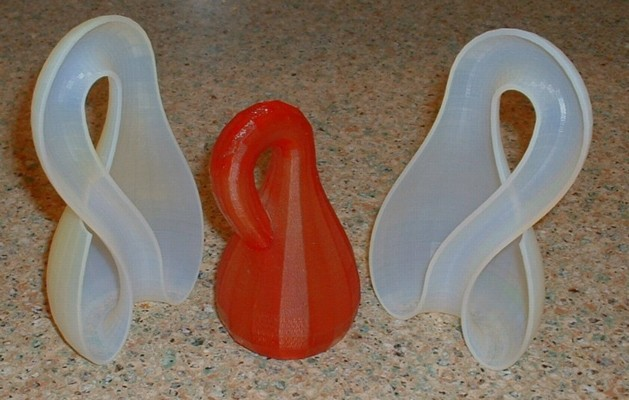
\includegraphics[width=0.7\linewidth]{klein-bottle}
	\end{center}
	This shows that the Klein bottle is a double co\fi
	(From \href{https://math.stackexchange.com/questions/1647836/what-can-be-said-about-the-leaves-of-a-regular-foliation}{StackExchange}) Consider $S^2\times I/\sim$ where we identify antipodal points in $S^2\times\{0\}$ and antipodal points in $S^2\times\{1\}$. It appears that this space is diffeomorphic to $\R P^3\#\R P^3$. Then the fibers of the quotient map are a foliation with leaves $S^2$ on $S^2\times(0,1)$ and $\R P^2$ on the ends.
\end{proof}
\printbibliography
\end{document}
